%!TEX root = ../report.tex
\section{System context}
The system context is a fundamental artifact in the software architecture of a system. Developing the system context view is important, because this view is used as a mechanism to trace back to the business context, and downstream to the functional and operational architecture.

\subsection{Diagram}
The system context diagram of the system is outlined in \autoref{fig:system-context-diagram}.

\begin{figure}[H]
\centering
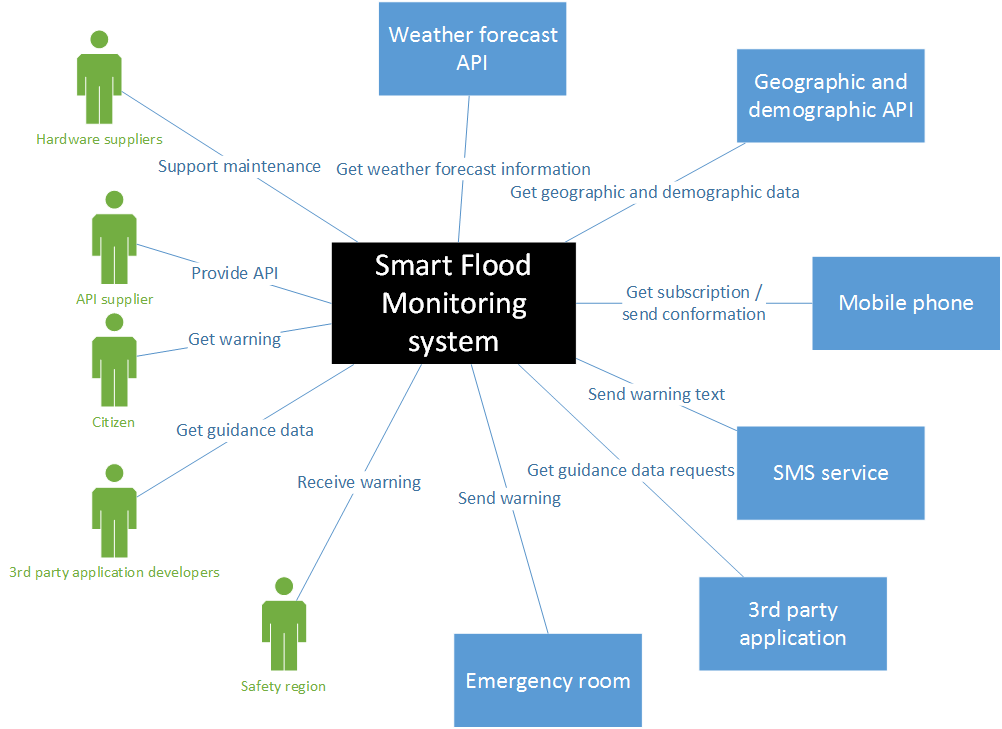
\includegraphics[keepaspectratio=true,width=0.7\textwidth]{images/system_context.png}
\caption{System context diagram}
\label{fig:system-context-diagram}
\end{figure}

\subsection{Users and Roles}
\begin{description}
	\item[Safety region] 
	\item[Citizens] In this system, citizens can be categorized into two group. First, citizens who do not subscribe to the service offered by the system. Second, citizens who subscribe the service. Indeed, Government will notify every citizens in affected areas. However, with subscription citizens can obtain more information regarding the flood and how to be safe.
	\item[Third party application developers] This user will also play an important role in case of floods. Emergency services will also be notified in case of imminent flood --- the government will notify them. Emergency services will also save the people and will be present in the affected areas.
	\item[Hardware suppliers] This user will also play an important role in case of floods. Emergency services will also be notified in case of imminent flood --- the government will notify them. Emergency services will also save the people and will be present in the affected areas.
\end{description} 

\subsection{External Systems}
\begin{description}
	\item[Weather Forecast API] The \ProjectName{} will also utilize weather forecast services from third party sources. This will help the system to predict upcoming flood. The system will also use several weather forecast provider to make sure that the weather information retrieved is reliable.
	\item[Geographic and demographic API] To monitor the conditions of waterways in the Netherlands, this system will gather all information about temperature, water pressure, and shifting. Together with weather forecast information collected from third party sources those information will be analyzed to predict upcoming flood.
	\item[Mobile phone] The \ProjectName{} will have an API that is accessible by other developers. By using information provided from the API, they are able to visualize data to make it more usable to broader users. 
	\item[SMS service] This system will communicate with subscribed citizens with their mobile devices. Government will also notify the citizens through mobile communication along with other information sources such as radio, television, and siren.
	\item[Third party application] This system will communicate to the government in case of imminent flood through API communications in the Internet. The information then will be forwarded to responsible stakeholders in the government.
	\item[Emergency room API] This system will communicate to the government in case of imminent flood through API communications in the Internet. The information then will be forwarded to responsible stakeholders in the government.
\end{description}

\subsection{Channels and Information Flows}
\begin{table}[!htbp]
	\centering
    \begin{tabular}{L{\tw{0.2}} L{\tw{0.4}}}
    \toprule
    \multicolumn{2}{c}{$SFM\: \Leftrightarrow \: Weather \: forecast \: API$} \\ \midrule
    \textbf{Description} & The \ProjectName{} gets temperature, water pressure, and shifting information from sensors in dykes. \\
    \textbf{Connection} & Wireless, Internet \\
    \textbf{Protocol} & 4G \\
    \textbf{Data Volume} & Real time \\
    \bottomrule
    \end{tabular}
\end{table}

\begin{table}[!htbp]
	\centering
    \begin{tabular}{L{\tw{0.2}} L{\tw{0.4}}}
    \toprule
    \multicolumn{2}{c}{$SFM \: \Leftrightarrow \: Geographic \: and \: demographic \: API$} \\ \midrule
    \textbf{Description} & The \ProjectName{} gets temperature, water pressure, and shifting information from sensors in dykes. \\
    \textbf{Connection} & Wireless, Internet \\
    \textbf{Protocol} & 4G \\
    \textbf{Data Volume} & Real time \\
    \bottomrule
    \end{tabular}
\end{table}

\begin{table}[!htbp]
	\centering
    \begin{tabular}{L{\tw{0.2}} L{\tw{0.4}}}
    \toprule
    \multicolumn{2}{c}{$SFM \: \Leftrightarrow \: Mobile \: Phone$} \\ \midrule
    \textbf{Description} & The \ProjectName{} gets temperature, water pressure, and shifting information from sensors in dykes. \\
    \textbf{Connection} & Wireless, Internet \\
    \textbf{Protocol} & 4G \\
    \textbf{Data Volume} & Real time \\
    \bottomrule
    \end{tabular}
\end{table}
\begin{table}[!htbp]
	\centering
    \begin{tabular}{L{\tw{0.2}} L{\tw{0.4}}}
    \toprule
    \multicolumn{2}{c}{$SFM \: \Leftrightarrow \: SMS \: Service$} \\ \midrule
    \textbf{Description} & The \ProjectName{} gets temperature, water pressure, and shifting information from sensors in dykes. \\
    \textbf{Connection} & Wireless, Internet \\
    \textbf{Protocol} & 4G \\
    \textbf{Data Volume} & Real time \\
    \bottomrule
    \end{tabular}
\end{table}
\begin{table}[!htbp]
	\centering
    \begin{tabular}{L{\tw{0.2}} L{\tw{0.4}}}
    \toprule
    \multicolumn{2}{c}{$SFM \: \Leftrightarrow \: Third \: party \: application$} \\ \midrule
    \textbf{Description} & The \ProjectName{} gets temperature, water pressure, and shifting information from sensors in dykes. \\
    \textbf{Connection} & Wireless, Internet \\
    \textbf{Protocol} & 4G \\
    \textbf{Data Volume} & Real time \\
    \bottomrule
    \end{tabular}
\end{table}
\begin{table}[!htbp]
	\centering
    \begin{tabular}{L{\tw{0.2}} L{\tw{0.4}}}
    \toprule
    \multicolumn{2}{c}{$SFM \: \Leftrightarrow \: Emergency \: room \: API$} \\ \midrule
    \textbf{Description} & The \ProjectName{} gets temperature, water pressure, and shifting information from sensors in dykes. \\
    \textbf{Connection} & Wireless, Internet \\
    \textbf{Protocol} & 4G \\
    \textbf{Data Volume} & Real time \\
    \bottomrule
    \end{tabular}
\end{table}


\subsection{Alternatives}

\subsubsection*{Wired Connections}
Sensors will send real time information about the dykes and waterways to the Sensor monitoring block. The system will mostly use wireless connection to push the information gathered by sensors. Wired connection can also be used to send the information. However, this option needs physical connection between sensor monitoring and the sensors itself which will make the production cost way bigger since there will be many sensors installed. Thus, the wireless connection is the most feasible method.
